\documentclass[11pt,preprint, authoryear]{elsarticle}

\makeatletter
\renewcommand\@biblabel[1]{}
\makeatother

\usepackage{lmodern}
%%%% My spacing
\usepackage{setspace}
\setstretch{1.2}
\DeclareMathSizes{12}{14}{10}{10}

% Wrap around which gives all figures included the [H] command, or places it "here". This can be tedious to code in Rmarkdown.
\usepackage{float}
\let\origfigure\figure
\let\endorigfigure\endfigure
\renewenvironment{figure}[1][2] {
    \expandafter\origfigure\expandafter[H]
} {
    \endorigfigure
}

\let\origtable\table
\let\endorigtable\endtable
\renewenvironment{table}[1][2] {
    \expandafter\origtable\expandafter[H]
} {
    \endorigtable
}


\usepackage{ifxetex,ifluatex}
\usepackage{fixltx2e} % provides \textsubscript
\ifnum 0\ifxetex 1\fi\ifluatex 1\fi=0 % if pdftex
  \usepackage[T1]{fontenc}
  \usepackage[utf8]{inputenc}
\else % if luatex or xelatex
  \ifxetex
    \usepackage{mathspec}
    \usepackage{xltxtra,xunicode}
  \else
    \usepackage{fontspec}
  \fi
  \defaultfontfeatures{Mapping=tex-text,Scale=MatchLowercase}
  \newcommand{\euro}{€}
\fi

\usepackage{amssymb, amsmath, amsthm, amsfonts}

\def\bibsection{\section*{References}} %%% Make "References" appear before bibliography


\usepackage[round]{natbib}

\usepackage{longtable}
\usepackage[margin=2.3cm,bottom=2cm,top=2.5cm, includefoot]{geometry}
\usepackage{fancyhdr}
\usepackage[bottom, hang, flushmargin]{footmisc}
\usepackage{graphicx}
\numberwithin{equation}{section}
\numberwithin{figure}{section}
\numberwithin{table}{section}
\setlength{\parindent}{0cm}
\setlength{\parskip}{1.3ex plus 0.5ex minus 0.3ex}
\usepackage{textcomp}
\renewcommand{\headrulewidth}{0.2pt}
\renewcommand{\footrulewidth}{0.3pt}

\usepackage{array}
\newcolumntype{x}[1]{>{\centering\arraybackslash\hspace{0pt}}p{#1}}

%%%%  Remove the "preprint submitted to" part. Don't worry about this either, it just looks better without it:
\makeatletter
\def\ps@pprintTitle{%
  \let\@oddhead\@empty
  \let\@evenhead\@empty
  \let\@oddfoot\@empty
  \let\@evenfoot\@oddfoot
}
\makeatother

 \def\tightlist{} % This allows for subbullets!

\usepackage{hyperref}
\hypersetup{breaklinks=true,
            bookmarks=true,
            colorlinks=true,
            citecolor=blue,
            urlcolor=blue,
            linkcolor=blue,
            pdfborder={0 0 0}}


% The following packages allow huxtable to work:
\usepackage{siunitx}
\usepackage{multirow}
\usepackage{hhline}
\usepackage{calc}
\usepackage{tabularx}
\usepackage{booktabs}
\usepackage{caption}


\newenvironment{columns}[1][]{}{}

\newenvironment{column}[1]{\begin{minipage}{#1}\ignorespaces}{%
\end{minipage}
\ifhmode\unskip\fi
\aftergroup\useignorespacesandallpars}

\def\useignorespacesandallpars#1\ignorespaces\fi{%
#1\fi\ignorespacesandallpars}

\makeatletter
\def\ignorespacesandallpars{%
  \@ifnextchar\par
    {\expandafter\ignorespacesandallpars\@gobble}%
    {}%
}
\makeatother

\newlength{\cslhangindent}
\setlength{\cslhangindent}{1.5em}
\newenvironment{CSLReferences}%
  {\setlength{\parindent}{0pt}%
  \everypar{\setlength{\hangindent}{\cslhangindent}}\ignorespaces}%
  {\par}


\urlstyle{same}  % don't use monospace font for urls
\setlength{\parindent}{0pt}
\setlength{\parskip}{6pt plus 2pt minus 1pt}
\setlength{\emergencystretch}{3em}  % prevent overfull lines
\setcounter{secnumdepth}{5}

%%% Use protect on footnotes to avoid problems with footnotes in titles
\let\rmarkdownfootnote\footnote%
\def\footnote{\protect\rmarkdownfootnote}
\IfFileExists{upquote.sty}{\usepackage{upquote}}{}

%%% Include extra packages specified by user

%%% Hard setting column skips for reports - this ensures greater consistency and control over the length settings in the document.
%% page layout
%% paragraphs
\setlength{\baselineskip}{12pt plus 0pt minus 0pt}
\setlength{\parskip}{12pt plus 0pt minus 0pt}
\setlength{\parindent}{0pt plus 0pt minus 0pt}
%% floats
\setlength{\floatsep}{12pt plus 0 pt minus 0pt}
\setlength{\textfloatsep}{20pt plus 0pt minus 0pt}
\setlength{\intextsep}{14pt plus 0pt minus 0pt}
\setlength{\dbltextfloatsep}{20pt plus 0pt minus 0pt}
\setlength{\dblfloatsep}{14pt plus 0pt minus 0pt}
%% maths
\setlength{\abovedisplayskip}{12pt plus 0pt minus 0pt}
\setlength{\belowdisplayskip}{12pt plus 0pt minus 0pt}
%% lists
\setlength{\topsep}{10pt plus 0pt minus 0pt}
\setlength{\partopsep}{3pt plus 0pt minus 0pt}
\setlength{\itemsep}{5pt plus 0pt minus 0pt}
\setlength{\labelsep}{8mm plus 0mm minus 0mm}
\setlength{\parsep}{\the\parskip}
\setlength{\listparindent}{\the\parindent}
%% verbatim
\setlength{\fboxsep}{5pt plus 0pt minus 0pt}



\begin{document}



%titlepage
\thispagestyle{empty}
\begin{center}
\begin{minipage}{0.75\linewidth}
    \centering
%Entry1
    {\uppercase{\huge COVID-19 Vaccine Lottery Field Experiment\par}}
    \vspace{2cm}
%Author's name
    {\LARGE \textbf{Cassandra Pengelly | 20346212}\par}
    \vspace{1cm}
%University logo
\begin{center}
    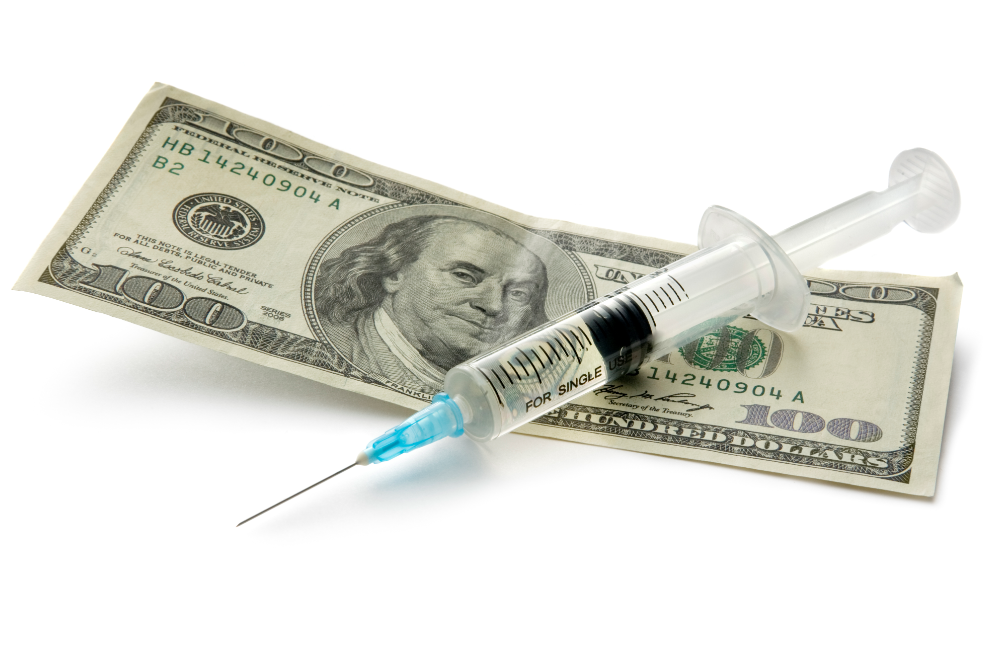
\includegraphics[width=0.9\linewidth]{Tex/logo.png}
\end{center}
\vspace{1cm}
%Supervisor's Details
\begin{center}
    {\LARGE Professor R. Burger\par}
    \vspace{1cm}
%Degree
    {\LARGE Behavioural Economics 871 Essay\par}
    \vspace{1cm}
%Institution
    {\LARGE 15 October 2021 \textbar{} Word Count: 2980\par}
    \vspace{1cm}
%Date
    {\large }
%More
    {\normalsize }
%More
    {\normalsize }
\end{center}
\end{minipage}
\end{center}
\clearpage


\begin{frontmatter}  %

\title{}

% Set to FALSE if wanting to remove title (for submission)


\vspace{1cm}





\vspace{0.5cm}

\end{frontmatter}


\renewcommand{\contentsname}{Table of Contents}
{\tableofcontents}

%________________________
% Header and Footers
%%%%%%%%%%%%%%%%%%%%%%%%%%%%%%%%%
\pagestyle{fancy}
\chead{}
\rhead{}
\lfoot{}
\rfoot{\footnotesize Page \thepage}
\lhead{}
%\rfoot{\footnotesize Page \thepage } % "e.g. Page 2"
\cfoot{}

%\setlength\headheight{30pt}
%%%%%%%%%%%%%%%%%%%%%%%%%%%%%%%%%
%________________________

\headsep 35pt % So that header does not go over title




\newpage

\hypertarget{introduction}{%
\section{\texorpdfstring{Introduction
\label{Introduction}}{Introduction }}\label{introduction}}

Coronavirus disease 2019 (COVID-19) has caused the largest public health
crisis, and economic disaster of the 21st century so far
(\protect\hyperlink{ref-bad}{Kadkhoda, 2021: 471}). According to the
\protect\hyperlink{ref-who}{World Health Organisation}
(\protect\hyperlink{ref-who}{2021}), COVID-19 has directly resulted in
4,859,277 deaths worldwide\footnote{As of 13 October 2021}, and its
impact on the global economy has been severe
(\protect\hyperlink{ref-bank}{World Bank, 2020}). Policymakers are in
urgent need of evidence-based strategies to contain the pandemic. As
\protect\hyperlink{ref-immun}{Fontanet \& Cauchemez}
(\protect\hyperlink{ref-immun}{2020: 583}) report, one critical
mechanism through which epidemics are controlled is herd immunity. Herd
immunity arises when a sufficiently large proportion of the population
achieves individual immunity to an infectious disease such that the
transmission chain of the disease is halted
(\protect\hyperlink{ref-bad}{Kadkhoda, 2021: 471}). One method of
establishing herd immunity is through vaccination programs
(\protect\hyperlink{ref-immun}{Fontanet \& Cauchemez, 2020: 583}).
Empirical evidence shows that vaccination strategies have helped subdue
COVID-19. For example, \protect\hyperlink{ref-erad}{Aldila, Samiadji,
Simorangkir, Khosnaw \& Shahzad} (\protect\hyperlink{ref-erad}{2021})
find COVID-19 vaccines to be effective in Indonesia. Other countries
have also implemented vaccine programs and the
\protect\hyperlink{ref-who}{World Health Organisation}
(\protect\hyperlink{ref-who}{2021}) reports that a total of
6,364,021,792 vaccine doses have been administered globally\footnote{As
  of 10 October 2021}.

In line with the international approach, South Africa has issued
vaccines in addition to social distancing and lockdown measures. The
South African government has stated that it aims to have 67\% of the
population vaccinated by the end of 2021
(\protect\hyperlink{ref-herd}{Department of Health, 2021a}). However,
many South Africans are hesitant to get the COVID-19 vaccine; the
\protect\hyperlink{ref-stat}{Department of Health}
(\protect\hyperlink{ref-stat}{2021b}) records that only 25\% of South
Africa's adult population has been fully vaccinated as of 11 October
2021. According to \protect\hyperlink{ref-cram}{Burger, Maughan-Brown,
Köhler, English \& Tameris} (\protect\hyperlink{ref-cram}{2021}), 20\%
of South Africans are concerned that COVID-19 vaccines are not safe, and
a significant portion of South Africans still have to be convinced to
take the vaccine\footnote{A sentiment report from
  \protect\hyperlink{ref-report}{Department of Health}
  (\protect\hyperlink{ref-report}{2021c}) shows an interesting break
  down of different communities' beliefs surrounding the vaccine}. While
there are different ways to encourage vaccine uptake, such as mandatory
vaccination or lump-sum transfers, insights from behaviourial economics
could provide a more cost-effective solution: a vaccine lottery.

This essay\footnote{This essay was written in R using the package
  Texevier by \protect\hyperlink{ref-Texevier}{Katzke}
  (\protect\hyperlink{ref-Texevier}{2017})} proposes a field experiment
to investigate whether different vaccine lotteries -- standard, regret
and referral -- could improve vaccination rates in South Africa. This
essay is structured as follows. Section \ref{lit} reviews the relevant
literature on behavioural economics and health interventions. Section
\ref{context} elaborates on the South African context. Section
\ref{design} describes the design of the experiment and discusses the
theory of change. Section \ref{treatment} outlines how the treatment
will be administered and the data collection process. Section \ref{pre}
gives a pre-analysis plan, and the final section (\ref{con}) concludes.

\hypertarget{behavioural-economics-and-health-interventions}{%
\section{\texorpdfstring{Behavioural Economics and Health Interventions
\label{lit}}{Behavioural Economics and Health Interventions }}\label{behavioural-economics-and-health-interventions}}

Health professionals and policymakers are increasingly turning to
behavioural economics to understand how people make health decisions and
how behavioural insights can be used to improve public health outcomes
(\protect\hyperlink{ref-health}{Loewenstein, Asch, Friedman, Melichar \&
Volpp, 2012: 1}). Neoclassical economics assumes that people are
perfectly rational, whereas behavioural economics uses psychology and
economic theory to create more realistic models of human decision-making
(\protect\hyperlink{ref-rabin}{Rabin, 2002}). People are subject to
certain biases and often make use of heuristics in their decision-making
process, which can lead to predictable errors in judgment
\protect\hyperlink{ref-prospect}{Kahneman \& Tversky}
(\protect\hyperlink{ref-prospect}{1979}). Behavioural economics
literature investigates how these biases can be combated to improve
welfare outcomes. \protect\hyperlink{ref-nudge}{Thaler \& Sunstein}
(\protect\hyperlink{ref-nudge}{2008}) introduced the idea of a
nudge\footnote{Nudge: an intervention that alters behaviour towards a
  desired action. In order for an intervention to qualify as a nudge, it
  should be cheap and easy to avoid
  (\protect\hyperlink{ref-nudge}{Thaler \& Sunstein, 2008}).} as a way
to guide people to make better choices. For example, changing the
default option for organ donation to be opt-in as opposed to explicit
consent could benefit potential donors (who were deterred by the
registration process) and save more lives
(\protect\hyperlink{ref-nudge}{Thaler \& Sunstein, 2008: 176}).

A similar type of nudge can be applied to flu vaccines. A study
conducted by \protect\hyperlink{ref-opt}{Chapman, Li, Colby \& Yoon}
(\protect\hyperlink{ref-opt}{2010}) found that vaccination rates
increased by 36\% under an opt-in default than under an opt-out
condition. \protect\hyperlink{ref-flu}{Madrian}
(\protect\hyperlink{ref-flu}{2014: 9}) proposes other interventions for
promoting vaccinations, e.g.~encouraging people to plan the time and
location they will receive their vaccination. This has been implemented
in South Africa for the COVID-19 vaccine: the government has sent out
SMS's reminding people to get vaccinated, and a self registration portal
has been set up for citizens to enroll in the Electronic Vaccination
Data System (EVDS\footnote{This portal can be seen as a type of
  commitment device, in addition to being a data collection mechanism.})
(\protect\hyperlink{ref-evds}{Republic of South Africa, 2021}).

Behavioural economic theory and empirical studies suggest that lotteries
can be a useful device for public health interventions. A lottery system
can be a cost-effective mechanism for changing behaviour compared to
direct transfers because people tend to overweight small probabilities.
This is a key insight from the seminal work by
\protect\hyperlink{ref-prospect}{Kahneman \& Tversky}
(\protect\hyperlink{ref-prospect}{1979: 286}) on prospect theory and
implies individuals overestimate their chances of winning a lottery.
\protect\hyperlink{ref-hiv}{Björkman Nyqvist, Corno, Walque \& Svensson}
(\protect\hyperlink{ref-hiv}{2018}) ran an experiment in Lesotho, where
participants were entered into a lottery, and they could win a cash
prize if they tested negative for sexually transmitted infections. HIV
incidence decreased by 21.4\% over two years because of the
intervention. The study found that the lottery was particularly
effective at targeting participants who were more prone to risky sexual
behaviour (\protect\hyperlink{ref-hiv}{Björkman Nyqvist, Corno, Walque
\& Svensson, 2018}). This supports the theory that risk-seeking
individuals value lotteries more.

The concepts of loss aversion, reference dependence and regret avoidance
can also be included in health interventions through a ``regret
lottery''. \protect\hyperlink{ref-prospect}{Kahneman \& Tversky}
(\protect\hyperlink{ref-prospect}{1979}) describe loss aversion as a
cognitive bias whereby people experience losses as more painful than the
pleasure they receive from an equivalent gain. Thus, people are more
willing to take on risk to avoid a loss, and are less risk-seeking when
pursuing gain (\protect\hyperlink{ref-prospect}{Kahneman \& Tversky,
1979: 268}). Reference dependence follows on from loss aversion and
suggests that people define gains and losses relative to a reference
point (\protect\hyperlink{ref-ref}{Tversky \& Kahneman, 1991: 1039}).
People are also subject to regret avoidance, where there is a
significant emotional cost attached to regret and people make decisions
to avoid regretting alternative decisions in the future
(\protect\hyperlink{ref-regret}{Bailey \& Kinerson, 2005}).

A regret lottery takes advantage of these three principles by entering
all participants into a lottery and the winner can claims the prize
contingent on some condition. If this condition is not met, a new winner
is selected. By entering all participants, people's reference point is
shifted to ``I have a chance at winning the lottery''. However, if a
person is not eligible to claim the prize because he does not meet the
required condition, he feels he has lost out. He is more likely to try
and meet the condition to minimise the pain of this loss. Additionally,
he will want to avoid the regret that would come from having missed the
opportunity to claim the prize. Several empirical papers investigate how
``regret lotteries'' can improve health behaviours.
\protect\hyperlink{ref-adhere}{Humphrey, Small, Jensen, Volpp, Asch, Zhu
\& Troxel} (\protect\hyperlink{ref-adhere}{2019}) analysed the effect of
a daily regret lottery on cholesterol-lowering, and heart medication
adherence, and found that the treatment group better adhered to their
medication regime than the control group. In a different study,
\protect\hyperlink{ref-regr}{Husain, Diaz, Schwartz, Parsons, Burg,
Davidson \& Kronish} (\protect\hyperlink{ref-regr}{2019}) found that
implementing a weekly electronic regret lottery increased adherence to a
self-monitoring study protocol.

Some states in America have run regret lotteries to encourage people to
get vaccinated against COVID-19. An unpublished paper by Thaler \emph{et
al} evaluates the effect of regret lotteries in Philadelphia
(\protect\hyperlink{ref-duck}{Gandhi, Milkman, Ellis, Graci, Gromet,
Mobarak, Buttenheim, Duckworth, Pope, Stanford, Thaler \& Volpp, 2021}).
The authors did not find convincing evidence that the regret lotteries
significantly increased first-dose vaccination rates for the treatment
groups\footnote{The authors acknowledge that there were some design
  flaws in the experiment that could be clouding the results.}.
Similarly disappointing results were found for a COVID-19 vaccine
lottery in Ohio (\protect\hyperlink{ref-ohio}{Walkey, Law \& Bosch,
2021}). To the best of my knowledge, there have been no studies on
COVID-19 vaccine lotteries in South Africa\footnote{It should be noted,
  however, that First National Bank is running a COVID-19 vaccine
  lottery for FNB customers, with total cash prizes amounting to R18
  million} - a gap which this experiment is intended to fill. This
experiment would also contribute to the empirical literature on
lotteries as public health interventions and the integration of
behavioural economics into public policy.

\hypertarget{the-south-african-context}{%
\section{\texorpdfstring{The South African Context
\label{context}}{The South African Context }}\label{the-south-african-context}}

A report by the \protect\hyperlink{ref-lotto}{National Lotteries
Commission} (\protect\hyperlink{ref-lotto}{2019}) on lottery habits
shows that 35\% of South Africans\footnote{Based on a sample of 3,090
  households randomly distributed across the country.} participated in
lottery activities in 2018 (\protect\hyperlink{ref-lotto}{National
Lotteries Commission, 2019: 78--79}). This high participation rate
supports the implementation of a vaccine lottery in South Africa, as
there is evidence of ``demand'' for lotteries. The average amount spent
on lottery activities was R156 per month, with average monthly lottery
winnings amounting to R110. A rational agent would not buy lottery
tickets due to the negative expected value (\(-\)R46). Yet people still
play the lotto, which suggests that South Africans may not be rational,
and behavioural economic insights are applicable\footnote{The gross
  revenue from gambling activities, excluding the National Lottery,
  amounted to R32.7 billion for the 2019 financial year
  (\protect\hyperlink{ref-gamble}{National Gambling Board, 2020: 3}).
  This represents 0.64\% of South Africa's 2019 nominal GDP (R5.1
  trillion) (\protect\hyperlink{ref-statsa}{Statistics South Africa,
  2020: 8}), which suggests that gambling is a lucrative market in South
  Africa and a lotto device could be an appropriate tool for
  incentivising behaviour.}.

Johnson \& Johnson (J\&J), Pfizer and AstraZeneca are all approved
COVID-19 vaccines in South Africa (\protect\hyperlink{ref-sah}{South
African Health Products Regulatory Authority, 2021}) and citizens have
to register on the EVID portal before receiving a vaccine. Some vaccines
require more than one dose. For this experiment, \emph{fully vaccinated}
refers to an individual who has had the maximum required doses of any
vaccine. \emph{Vaccinated} refers to an individual who has had 1 shot of
any vaccine. According to the \protect\hyperlink{ref-stat}{Department of
Health} (\protect\hyperlink{ref-stat}{2021b}), 34\% of South Africans
are vaccinated, while 25\% are fully vaccinated. These low numbers
indicate that an intervention is necessary to improve vaccination rates
if South Africa wants to achieve herd immunity. Table \ref{tab1} below
gives a breakdown of vaccination rates.

\begin{table}[H]
\centering
\begin{tabular}{llll}
  \toprule
Province & Total Adults Vaccinated & Adult Population & Percentage Vaccinated \\ 
  \midrule
Eastern Cape & 1 603 045 & 4 099 543 & 39\% \\ 
  Free State & 735 696 & 1 914 521 & 38\% \\ 
  Gauteng & 3 523 373 & 11 311 326 & 31\% \\ 
  KwaZulu-Natal & 2 170 526 & 7 219 795 & 30\% \\ 
  Limpopo & 1 437 846 & 3 695 801 & 39\% \\ 
  Mpumalanga & 831 759 & 3 039 520 & 27\% \\ 
  North West & 835 206 & 2 693 247 & 31\% \\ 
  Northern Cape & 290 962 & 847 545 & 34\% \\ 
  Western Cape & 2 141 933 & 4 976 903 & 43\% \\ 
  Total & 13 570 346 & 39 798 201 & 34\% \\ 
   \bottomrule
\end{tabular}
\caption{Vaccination Statistics \label{tab1}} 
\end{table}

\hypertarget{experiment-design}{%
\section{\texorpdfstring{Experiment Design
\label{design}}{Experiment Design }}\label{experiment-design}}

\hypertarget{sample}{%
\subsection{Sample}\label{sample}}

The sample used in this experiment will be the same sample used for the
Coronavirus Rapid Mobile Survey (NIDS-CRAM)\footnote{NIDS-CRAM was
  created to build a representative data set of the South African
  population to inform decision-making for the pandemic}
(\protect\hyperlink{ref-nids}{Ingle, 2021}). There have been five waves
of NIDS-CRAM surveys, with wave 5 comprising 5,862 people\footnote{Suveyed
  over April to May 2021} (\protect\hyperlink{ref-nids}{Ingle, 2021:
14}). Wave 3 comprised 8,157 potential participants, of which 6,130 were
interviewed. For this experiment, the 8,157 people from wave 3 will be
contacted and asked to participate in wave 6. We can expect between
5,500-6,200 people to participate, given the previous attrition rates in
NIDS-CRAM.

A conservative sample size of 5,500 and a vaccination proportion of
34\%, leaves 3630 eligible participants for the study\footnote{Since we
  are interested in unvaccinated individuals}. This sample will be split
into 4 groups of equal size (907), and randomised such that each group
has a similar distribution of participants in terms of age, race, health
status and gender, as proposed by \protect\hyperlink{ref-random}{Duflo,
Glennerster \& Kremer}
(\protect\hyperlink{ref-random}{2007})\footnote{This randomisation
  serves to ensure groups are comparable, and eliminate bias in
  treatment assignments.}. One group is randomly chosen to be the
control group, and the other 3 groups are randomly allocated to
different lottery treatments. There will be 1 lottery a month for each
treatment group, which will run for three months. There will be 9
lotteries in total, with 3 lotteries every month. Lottery winners
receive a cash prize of R1,000,000.

\hypertarget{treatment-groups}{%
\subsection{\texorpdfstring{Treatment Groups
\label{group}}{Treatment Groups }}\label{treatment-groups}}

For the first treatment group, if an individual has received a
vaccination shot within a given month, she will be entered into that
month's vaccine lottery. At the end of the month, a winner is randomly
selected; winners are privately contacted and receive a cash
prize\footnote{Once it is verified that the winner has indeed been
  vaccinated.}. The second lottery is a regret lottery. Every individual
in the group is entered into a monthly lottery but an individual may
only claim her prize if she has been vaccinated in that month. At month
end, a winner is randomly drawn. If the winner has been vaccinated, she
will be privately notified and receives a cash prize. If the winner has
not been vaccinated, she will receive a ``regret message'' stating that
she would have won the cash prize if she had been vaccinated; and a new
winner is drawn from the lottery.

The final treatment is a ``referral lottery''. An individual is entered
into the monthly lottery if 2 conditions are met: he is vaccinated, and
he refers a friend to get vaccinated and the friend gets vaccinated.
Both the individual from the treatment group and his friend are entered
into the lottery. At the end of the month, a winner is selected, and
once he and his referral partner are verified to be vaccinated, he will
be notified. An individual can refer more than one friend to be
vaccinated in any given month. However, only individuals from the
treatment group can refer friends\footnote{i.e.~people outside of group
  3 will not be entered into the lottery for referring others to get
  vaccinated}. Group 3 participants may not refer any person in the
control group or in group 1 or group 2 (to avoid contamination).

Whenever a lottery is won, it will be announced via SMS to all
participants in the relevant treatment group. The amount of the lottery
prize and the winner's province will also be included in the
SMS\footnote{This serves as a reminder of how large the cash prize is,
  and including the winner's province makes winning seem more tangible}.
Group 2's SMS will include a reminder that only vaccinated individuals
are eligible to win the lottery. Group 3's SMS will include a reminder
that participants can refer as many friends as they like to be eligible
for the following month's lottery. All SMS's will end with: ``Thank you
for vaccinating and keeping our country safe!'' as one final nudge to
encourage/guilt participants to vaccinate.

Table \ref{tab2} summarises the different treatments arms.

\begin{table}[H]
\centering
\begin{tabular}{ll}
  \toprule
Group & Treatment \\ 
  \midrule
Control & No lottery \\ 
  Group 1 & Individual is entered into a lottery once they are vaccinated \\ 
  Group 2 & Everyone in the group is entered into a lottery; only vaccinated individuals can \\ 
   & claim the prize \\ 
  Group 3 & Individual is entered if she is vaccinated and refers a friend, who gets vaccinated \\ 
   \bottomrule
\end{tabular}
\caption{Treatment Summary \label{tab2}} 
\end{table}

\hypertarget{theory-of-change}{%
\subsection{Theory of Change}\label{theory-of-change}}

The decisions and actions associated with getting vaccinated appear
deceptively simple but are the result of a complex series of behaviours
(\protect\hyperlink{ref-decide}{Brewer, Chapman, Rothman, Leask \&
Kempe, 2017: 154}). To design an intervention to increase vaccinations,
we need to understand who would be affected by the intervention. There
are two groups for whom any treatment is irrelevant: people who would
always choose to get vaccinated, and those who would never get
vaccinated. We are interested in identifying a group who would not get
vaccinated without intervention but with treatment would get vaccinated.
It is plausible that a standard lottery intervention would be appealing
to risk-on individuals (\protect\hyperlink{ref-hiv}{Björkman Nyqvist,
Corno, Walque \& Svensson, 2018}) and could convince them to vaccinate.
Even though the vaccine is free in South Africa, poorer individuals may
still be reluctant to incur the frictional costs of getting vaccinated
(such as transport costs). A lottery intervention could compensate for
such costs and incentivise vaccination, especially if such individuals
overweight small probabilities (see \ref{lit}).

If there are individuals who are willing to get vaccinated but
procrastinate (e.g.~naïve hyperbolic discounters), a lottery deadline
could help overcome the procrastination problem. Additionally, a lottery
could solve the herd immunity free-riding problem. A regret lottery
(treatment 2) would incentivise vaccination among individuals who
experience reference dependence, loss aversion and regret avoidance. We
would expect vaccination rates to be higher under treatment 2 compared
to treatment 1 since a regret lottery has all the same qualities of a
standard lottery, and additional incentives.

Treatment 3 uses aligned incentives\footnote{I like to think of
  treatment 3 as a positive-sum pyramid scheme} and social pressure to
encourage vaccinations. Both the friend and the referring individual get
a payoff from being vaccinated because of the lottery entry. However,
neither can enter the lottery without the other getting vaccinated,
which creates the pressure for each to get vaccinated as soon as
possible to avoid disappointing the other. Vaccination incentives are
now also a function of the social preferences of group 3 and their
friends. It is reasonable to assume that the introduction of a lottery
would not deter someone from getting vaccinated, who would have got
vaccinated otherwise. Thus, we would expect to see higher vaccination
rates for all three treatment groups compared to the control group.

\hypertarget{treatment-and-data}{%
\section{\texorpdfstring{Treatment and Data
\label{treatment}}{Treatment and Data }}\label{treatment-and-data}}

The two main partner institutions for this field experiment would be the
Department of Health, and the CRAM team\footnote{The CRAM project is
  supported by the Department of Planning Monitoring and Evaluation
  (DPME), the Research on Socioeconomic Policy (RESEP) group at
  Stellenbosch University, and the Southern Africa Labour and
  Development Research Unit (SALDRU) at UCT.}. Vaccine data is collected
by health professionals at the designated vaccination sites. The EVDS
captures a vaccinee's personal information\footnote{Names, Identity
  Number, medical aid details, residential address, email address, phone
  numbers, employment details, professional category, and health status.}
as well as the vaccine date and details. The only additional information
needed for the experiment is the name, ID number, and phone number of
the referring individual (under treatment 3). The person receiving the
vaccine is responsible for supplying these details to the vaccine
administrator. The agent who collected the information of the winning
person from group 3's lottery will receive R10,000. This is an incentive
for healthcare workers to correctly capture referral details.

The other data collection mechanism occurs through the NIDS-CRAM survey
(\protect\hyperlink{ref-quest}{Spaull, Posel, Wills, Makaluza, Daniels,
Burger, Burger, Berg, Ranchhod, Ingle, Brophy \& Carel, 2021}). Two
extra questions will be added to the original survey: ``How often do you
buy lotto tickets?'' and ``How often do you participate in gambling
activities?''. An additional survey section is needed to record the
personal information of the referred friends for group 3. This acts as a
second check for the referral information collected by healthcare
workers. It is assumed that the marginal cost of adding this section and
the two questions to the survey is negligible. This experiment is
designed to harness existing data collecting processes to reduce costs
and exploit the existing NIDS-CRAM time series data.

Funding for the experiment would need to cover: R9,000,000 for the cash
prizes, the admin fees associated with the SMS program and award
disbursement, and R30,000 for incentive fees for the people who capture
the winner's information from group 3's lottery. Potential funding
sources include the COVID-19 Africa Rapid Grant Fund administered by the
NRF, government funding, and private donors such as the Allan \& Gill
Gray Philanthropy.

\hypertarget{pre-analysis-plan}{%
\section{\texorpdfstring{Pre-analysis Plan
\label{pre}}{Pre-analysis Plan }}\label{pre-analysis-plan}}

First, a balance test should be employed to check that randomisation was
successful. If the F-test is not significant, then we know that the
covariates cannot be used to predict the treatment status, and we can
conclude that the covariates are balanced among treatment groups and the
sample has been randomised. To estimate the average treatment effect, an
OLS regression would be run with the outcome variable as the number of
first-dose vaccinations. The exogenous variables would include a dummy
variable for each of the treatment groups (which takes a value of 1 for
the treatment group and 0 otherwise) and a vector of covariates to
control for gender, age, health, income and education (this information
is captured in the NIDS-CRAM questionnaire). If the coefficients of the
dummy variables are positive and statistically significant, we can infer
that a lottery treatment improved vaccine uptake. A second OLS model
could include a control variable for how risk-seeking an individual is,
using the answers to the lottery and gambling questions as a proxy for
people's risk preferences. Interaction effects of the covariates with
the dummy variables could be included for a more comprehensive
understanding of how lottery incentives work for different individuals.
For all of the regressions, the standard robustness checks should be
applied.

A difference-in-difference regression approach could also be taken,
comparing monthly vaccinations per 100 individuals over time in the
control group, with the monthly per-100 vaccinations for each of the
treatment groups. Alternatively, a logit model could be used, where the
outcome variable is 1 if an individual is vaccinated and 0 otherwise;
the exogenous variables would include dummies for the different
treatment groups and a vector of covariates. For each model, it should
be assessed whether the estimates (and subgroup heterogeneity) are
consistent with the theory of change. Since most people are subject to
loss aversion and the other behavioural biases that drive the success of
vaccine lotteries, it stands to reason that the results of the empirical
analysis have external validity. Although, this makes no normative
assessment of whether vaccine lotteries are the most efficient use of
funding for incentivising vaccination.

\hypertarget{conclusion}{%
\section{\texorpdfstring{Conclusion
\label{con}}{Conclusion }}\label{conclusion}}

The behavioural literature and empirical studies show that lotteries can
be an effective method to incentivise vaccine take-up, and South
Africans appear to be well-primed for such a health intervention. This
field experiment is designed to test this hypothesis.

\newpage

\hypertarget{references}{%
\section*{References}\label{references}}
\addcontentsline{toc}{section}{References}

\hypertarget{refs}{}
\begin{CSLReferences}{1}{0}
\leavevmode\hypertarget{ref-erad}{}%
Aldila, D., Samiadji, B.M., Simorangkir, G.M., Khosnaw, S.H. \& Shahzad,
M. 2021. Impact of early detection and vaccination strategy in COVID-19
eradication program in jakarta, indonesia. \emph{BMC Research Notes}.
14(1):1--7.

\leavevmode\hypertarget{ref-regret}{}%
Bailey, J.J. \& Kinerson, C. 2005. Regret avoidance and risk tolerance.
\emph{Journal of Financial Counseling and Planning}. 16(1):23.

\leavevmode\hypertarget{ref-hiv}{}%
Björkman Nyqvist, M., Corno, L., Walque, D. de \& Svensson, J. 2018.
Incentivizing safer sexual behavior: Evidence from a lottery experiment
on HIV prevention. \emph{American Economic Journal: Applied Economics}.
10(3):287--314.

\leavevmode\hypertarget{ref-decide}{}%
Brewer, N.T., Chapman, G.B., Rothman, A.J., Leask, J. \& Kempe, A. 2017.
Increasing vaccination: Putting psychological science into action.
\emph{Psychological Science in the Public Interest}. 18(3):149--207.

\leavevmode\hypertarget{ref-cram}{}%
Burger, R., Maughan-Brown, B., Köhler, T., English, R. \& Tameris, M.
2021. \emph{A shot in the arm for south africa - increased openness to
accepting a COVID-19 vaccine: Evidence from NIDS-CRAM waves 4 and 5}.
National Income Dynamics Study (NIDS) -- Coronavirus Rapid Mobile Survey
(CRAM). {[}Online{]}, Available: \url{https://cramsurvey.org/reports/}.

\leavevmode\hypertarget{ref-opt}{}%
Chapman, G.B., Li, M., Colby, H. \& Yoon, H. 2010. Opting in vs opting
out of influenza vaccination. \emph{JAMA}. 304(1):43--44.

\leavevmode\hypertarget{ref-stat}{}%
Department of Health. 2021b. \emph{Latest vaccine statistics}. Republic
of South Africa. {[}Online{]}, Available:
\url{https://sacoronavirus.co.za/latest-vaccine-statistics/}.

\leavevmode\hypertarget{ref-herd}{}%
Department of Health. 2021a. \emph{COVID-19 coronavirus vaccine}.
Republic of South Africa. {[}Online{]}, Available:
\url{https://www.gov.za/covid-19/vaccine/vaccine}.

\leavevmode\hypertarget{ref-report}{}%
Department of Health. 2021c. \emph{South africa COVID-19 and vaccine
social listening report}. Republic of South Africa. {[}Online{]},
Available:
\url{https://sacoronavirus.b-cdn.net/wp-content/uploads/2021/10/SA-social-listening-report-5-Oct-2021.pdf}.

\leavevmode\hypertarget{ref-random}{}%
Duflo, E., Glennerster, R. \& Kremer, M. 2007. Using randomization in
development economics research: A toolkit. \emph{Handbook of development
economics}. 4:3895--3962.

\leavevmode\hypertarget{ref-immun}{}%
Fontanet, A. \& Cauchemez, S. 2020. COVID-19 herd immunity: Where are
we? \emph{Nature reviews. Immunology}. 20:583--584.

\leavevmode\hypertarget{ref-duck}{}%
Gandhi, L., Milkman, K.L., Ellis, S., Graci, H., Gromet, D., Mobarak,
R., Buttenheim, A., Duckworth, A., et al. 2021. An experiment evaluating
the impact of large-scale, high-payoff vaccine regret lotteries.
{[}Online{]}, Available: \url{http://dx.doi.org/10.2139/ssrn.3904365}.

\leavevmode\hypertarget{ref-adhere}{}%
Humphrey, C.H., Small, D.S., Jensen, S.T., Volpp, K.G., Asch, D.A., Zhu,
J. \& Troxel, A.B. 2019. Modeling lottery incentives for daily
adherence. \emph{Statistics in Medicine}. 38(15):2847--2867.

\leavevmode\hypertarget{ref-regr}{}%
Husain, S.A., Diaz, K.M., Schwartz, J.E., Parsons, F.E., Burg, M.M.,
Davidson, K.W. \& Kronish, I.M. 2019. Behavioral economics
implementation: Regret lottery improves mHealth patient study adherence.
\emph{Contemporary Clinical Trials Communications}. 15:100387.

\leavevmode\hypertarget{ref-nids}{}%
Ingle, B., K. 2021. \emph{National income dynamics study -- coronavirus
rapid mobile survey (NIDS-CRAM) 2020 - 2021 panel user manual.} Cape
Town: Southern Africa Labour; Development Research Unit: Bureau for
Economic Research.

\leavevmode\hypertarget{ref-bad}{}%
Kadkhoda, K. 2021. Herd immunity to COVID-19: Alluring and elusive.
\emph{American Journal of Clinical Pathology}. 155(4):471--472.

\leavevmode\hypertarget{ref-fast}{}%
Kahneman, D. 2011. \emph{Thinking, fast and slow}. Macmillan.

\leavevmode\hypertarget{ref-prospect}{}%
Kahneman, D. \& Tversky, A. 1979. Prospect theory: An analysis of
decision under risk. \emph{Econometrica}. 47(2):263--291.

\leavevmode\hypertarget{ref-Texevier}{}%
Katzke, N.F. 2017. \emph{{Texevier}: {P}ackage to create elsevier
templates for rmarkdown}. Stellenbosch, South Africa: Bureau for
Economic Research.

\leavevmode\hypertarget{ref-health}{}%
Loewenstein, G., Asch, D., Friedman, J., Melichar, L. \& Volpp, K. 2012.
Can behavioural economics make us healthier? \emph{BMJ (Clinical
research ed.)}. 344:e3482.

\leavevmode\hypertarget{ref-flu}{}%
Madrian, B. 2014. Applying insights from behavioral economics to policy
design. {[}Online{]}, Available: \url{http://dx.doi.org/10.3386/w20318}.

\leavevmode\hypertarget{ref-gamble}{}%
National Gambling Board. 2020. \emph{National gambling statistics:
Casinos, bingo, limited pay-out machines and betting on horse racing and
sport offered by bookmakers and totalisators. Audited statistics:2019/20
financial year}. {[}Online{]}, Available:
\url{https://www.ngb.org.za/SiteResources/documents/2020-21/Stats\%20Presentation\%20FY2019-20\%20pdf.pdf}.

\leavevmode\hypertarget{ref-lotto}{}%
National Lotteries Commission. 2019. \emph{2019 integrated report}.
{[}Online{]}, Available:
\url{http://www.nlcsa.org.za/ir/ir2019/NLC_ir2019/downloads/nlc-full.pdf\#view=Fit}.

\leavevmode\hypertarget{ref-rabin}{}%
Rabin, M. 2002. A perspective on psychology and economics.
\emph{European economic review}. 46(4-5):657--685.

\leavevmode\hypertarget{ref-evds}{}%
Republic of South Africa. 2021. \emph{Electronic vaccination data system
(EVDS) self registration portal}. {[}Online{]}, Available:
\url{https://www.gov.za/covid-19/vaccine/evds}.

\leavevmode\hypertarget{ref-sah}{}%
South African Health Products Regulatory Authority. 2021. \emph{MEDIA
RELEASE ON THE APPROVAL PROCESS OF COVID VACCINES}. {[}Online{]},
Available:
\url{https://www.sahpra.org.za/wp-content/uploads/2021/07/SAHPRA-CovidVaccineApproval_Media-Release_1July2021_FINAL.pdf}.

\leavevmode\hypertarget{ref-quest}{}%
Spaull, N., Posel, D., Wills, G., Makaluza, N., Daniels, R., Burger, R.,
Burger, R., Berg, S. van der, et al. 2021. \emph{NIDS-CRAM
questionnaire. Wave 5}. {[}Online{]}, Available:
\url{https://cramsurvey.org/wp-content/uploads/2021/07/NIDS-CRAM_Wave5_Questionnaire.pdf}.

\leavevmode\hypertarget{ref-statsa}{}%
Statistics South Africa. 2020. Gross domestic product fourth quarter
2019: STATISTICAL RELEASE P0441. {[}Online{]}, Available:
\url{https://www.statssa.gov.za/publications/P0441/P04414thQuarter2019.pdf}.

\leavevmode\hypertarget{ref-nudge}{}%
Thaler, R. \& Sunstein, C. 2008. \emph{Nudge: Improving decisions about
health, wealth, and happiness.} New Haven, CT: Yale University Press.

\leavevmode\hypertarget{ref-khan}{}%
Tversky, A. \& Kahneman, D. 1974. Judgment under uncertainty: Heuristics
and biases. \emph{Science}. 185(4157):1124--1131.

\leavevmode\hypertarget{ref-ref}{}%
Tversky, A. \& Kahneman, D. 1991. Loss aversion in riskless choice: A
reference-dependent model. \emph{The Quarterly Journal of Economics}.
106(4):1039--1061. {[}Online{]}, Available:
\url{http://www.jstor.org/stable/2937956}.

\leavevmode\hypertarget{ref-ohio}{}%
Walkey, A.J., Law, A. \& Bosch, N.A. 2021. Lottery-based incentive in
ohio and COVID-19 vaccination rates. \emph{JAMA}. 326(8):766--767.

\leavevmode\hypertarget{ref-bank}{}%
World Bank. 2020. \emph{The global economic outlook during the COVID-19
pandemic: A changed world}. {[}Online{]}, Available:
\url{https://www.worldbank.org/en/news/feature/2020/06/08/the-global-economic-outlook-during-the-covid-19-pandemic-a-changed-world}.

\leavevmode\hypertarget{ref-who}{}%
World Health Organisation. 2021. \emph{WHO coronavirus (COVID-19)
dashboard}. {[}Online{]}, Available:
\url{https://covid19.who.int/table}.

\end{CSLReferences}

\bibliography{Tex/ref}





\end{document}
